%------------------------------------------------------------------------
%Editar Diplomado
\hypertarget{cv:eliminarProyecto}{\section{Eliminar Proyecto de administrador}} \label{sec:eliminarProyecto}

	Esta funcionalidad le permitirá eliminar un proyecto que no se completo o se canceló. Para eliminar un proyecto es necesario que no tenga casos de uso asociados.

		\subsection{Procedimiento}

			%Pasos de procedimiento
			\begin{enumerate}
	
			\item Oprima el botón \IUBotonEliminar{} de un registro existente de la pantalla \ref{fig:GestionarProyectosAdmin} ''Gestionar Proyectos de Administrador''.
	
			\item Se mostrará el mensaje \ref{fig:confirmaEliminaProyecto} sobre la pantalla \ref{fig:GestionarProyectosAdmin} ''Gestionar Proyectos de Administrador''.
			
			%Pantalla
			\begin{figure}[htbp!]
				\begin{center}
					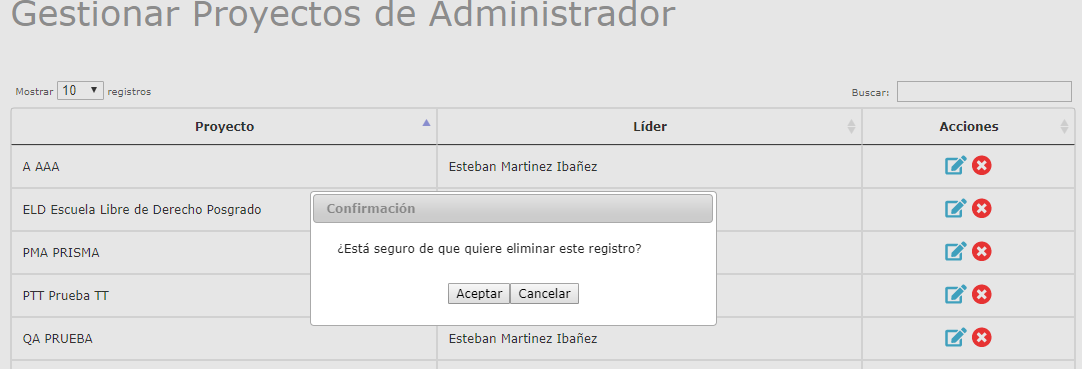
\includegraphics[scale=0.6]{roles/administrador/proyectosAdmin/gestionarproyectosAdmin/pantallas/IU2-3MSG10}
					\caption{MSG de Confirmación}
					\label{fig:confirmaEliminaProyecto}
				\end{center}
			\end{figure}
						
			\item Oprima el botón \IUAceptar.
			
			\item Se mostrará el mensaje \ref{fig:proyectoEliminado} en la pantalla \ref{fig:GestionarProyectosAdmin} ''Gestionar Proyectos de Administrador''.
			
			\begin{figure}[htbp!]
				\begin{center}
					
\includegraphics[scale=0.6]{roles/administrador/proyectosAdmin/gestionarproyectosAdmin/pantallas/IU2-3MSG1}
					\caption{MSG: Salón Eliminado}
					\label{fig:proyectoEliminado}
				\end{center}
			\end{figure}
			\end{enumerate}